\chapter{Introduction}
\label{1}
Microfluidic devices have presented an attractive platform to researchers in recent years for performing studies into a wide variety of microbiological processes. Bacteria adhesion, for example, is one of the interested processes to be studied. This thesis project is developed in the framework of microfluidic technology to build a microfluidic platform which may be used for future work studying the bacteria adhesion features at the solid-liquid interfaces. In this chapter the motivation of designing this microfluidic platform and the advantages of this design is discussed. The aim of this thesis work as well as the frame of the thesis will also be explained. Moreover, a brief description of the approach for achieving the goal is presented.

\section{Motivation}
\label{1_1}
The aim of this master thesis work is to design a modular microfluidic platform to study the transport and adhesion mechanism of individual bacteria on both solid and semi-permeable surfaces and their relation to the kinetics and statistics of bacteria deposition in a flow in microfluidic channels. When the bacteria-containing suspension flows in a microchannel, the transported bacteria will either adhere to the wall or slide or roll downstream when it reaches the wall, depending on the surface properties and hydrodynamic conditions. Such adhesion can lead to surface colonization by bacteria and the formation of biofilms (biofilms are sessile microbial communities growing on surfaces). In certain scenarios the growth of these biofilms might be desired at certain locations in a microfluidic system, e.g. for cultivation studies, while in other scenarios this growth can lead to unwanted channel blockage. Therefore the study of such micro-processes is a topic of great interest.\\

When the microchannel is formed by impermeable walls shown in  \autoref{figure1_1} (a), there is only cross flow within the channel. Some studies about the bacteria adhesion feature under such scenario are already done \cite{elimelech2013particle} \cite{levich1962physicochemical}. However, when one side of the wall is replaced by semi-permeable membranes shown in \autoref{figure1_1} (b), the permeate flow is introduced and thus the downstream movement such as sliding and rolling would be affected by the introduced normal drag force. In particular, when the depth of the microchannel varies along its length (\autoref{figure1_2}), the flow velocity will also change along the length of the channel in a single test, leading to the variation of the tangential shear stress. These hydrodynamic variations may provide opportunities to setup a model to study the adhesion mechanism of bacteria at surfaces with different flow rate and multiple flow components.


\begin{figure}[ht]%
\centering
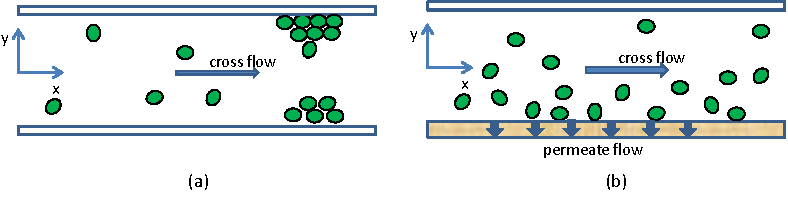
\includegraphics[width=0.8\textwidth]{figures/introduction/figure1_1}%
\caption{(a) Microchannel with impermeable walls. (b) Microchannel with semi-permeable wall on one side.}%
\label{figure1_1}%
\end{figure}

\begin{figure}[ht]%
\centering
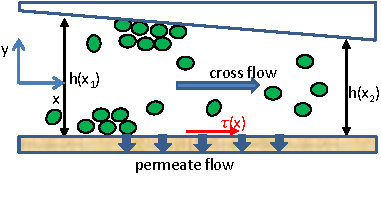
\includegraphics[width=0.4\textwidth]{figures/introduction/figure1_2}%
\caption{Microchannel with variable channel depth.}%
\label{figure1_2}%
\end{figure}

Microfluidic devices, in which low volume of fluids are moved, separated or processed, are now widely used in the research of fluid properties and many kinds of micro-processes in the fluids. On the one hand, the high surface-to-volume ratios in fluids can provide contact area for substance like bacteria to interact with the channel walls, which makes it sometimes easier to obtain measureable and even observable micro-processes such as growing or adhesion of bacteria to the channel walls. On the other hand, small volumes are also easier to be controlled under specific process conditions such as pressure and flow rate. Thus microfluidic devices can provide platforms for generating well-controlled hydrodynamic properties of the flow for studying complex coupled micro-processes in the microchannels. 


\subsection{Microfluidic Platform for Testing of Bacteria Adhesion Features}
\label{1_1_1}
As illustrated in the former section, in this master thesis a microfluidic platform is designed to study the adhesion mechanism of bacteria on both solid and semi-permeable surfaces. The semi-permeable surface in this thesis work is achieved by nanofiltration membranes and the adhesion features of the bacteria during separation are to be studied. This microfluidic platform is supposed to provide an ideal approach for in-depth direct investigation of the microscopic processes that occur at the membrane surface during separations. 

\subsection{Reusable and Resealable for High Pressure Applications}
\label{1_1_2}
Handling fluids at high pressures is quite demanding. Firstly, the forces present must be considered in order to ensure that the structural strength of the device and material is sufficient. Secondly, interfacing and sealing need to be accounted for, usually solved at macro scale by welding and the use of O-rings. Thus it is meaningful and at the same time of great challenge to develop a microfluidic platform for high pressure applications. There are two conventional packaging methods for the housing in high pressure applications, one of which is permanent integrated connections including epoxy gluing, metal soldering or glass brazing \cite{marre2010design}. These connections are able to withstand high pressures in particular designs \cite{blom2001local}. However, such high pressure performance is achieved at the expense of losing the versatility and the reversibility. The non-permanent modular connection methods can also be used for packaging especially for those microfluidic systems which can be assembled and disassembled for multiple times. These connection methods are involved with different kinds of gaskets which can be reused after disassembling and do not hurt the microfluidic system at the same time.\\

In our case, the separation process is achieved by filtering under high pressure with the NF membrane. The pressure will push water molecules through the NF membrane while the charged ions will be repelled by the electrical surface charges on the NF membrane. Bacteria, due to their large physical size, can also not pass through the NF membrane since the mesh size of the NF membrane is within the nanometer range. The deposition and adhesion features of the bacteria are to be studied so that the NF membrane needs to be replaced after a single test by a new piece of NF membrane and this leads to the disassembling and reassembling of the microfluidic platform. Therefore it is of great importance to keep a good sealing performance and steady mechanical stability of the housing after reassembling to make the platform reusable and resealable. 


\subsection{Laser Rapid Prototyping for Flexible Channel Fast Fabrication}
\label{1_1_3}
Rapid prototyping (RP) is a term which embraces a range of new technologies for producing accurate parts directly from three-dimensional computer aided design (CAD) data \cite{pham1998comparison}. This means that the designers have the freedom to produce physical models of their drawings more frequently, allowing them to check the assembly and function of the design. As a result, errors are minimized and the developing cost and lead times are significantly saved. \\

Processing technologies regarding processing microstructures may be divided broadly into those involving the addition of material and those involving its removal \cite{lehmann1995laser}. The main technology for material removal is lithography and etching techniques which can manufacture high quality three-dimensional microstructures. However, these techniques require photo masks to be made before the microstructures can be produced, and the production itself consists of many complicated and time-consuming steps. Besides, any structural redevelopment would require the redesign of the masks. Therefore such techniques are only economical for mass production of a single design that does not need any further development. In the case of this thesis work, however, the design of the microchannel needs to be quite flexible in order to test the filtration features under different channel geometries. As a result, the etching techniques are not the optimal processing techniques with respect to the application in this thesis work.\\

Laser rapid prototyping (LRP) technique developed in this thesis work is defined as laser indirect cut into the work piece. Repeating the laser processing path will simply result in the variation of cutting depth and this gives the possibility for three-dimensional machining. With the use of computer-aided design the structure data could be transferred directly to the laser machine and can be processed within tens of minutes. Therefore high design flexibility can be achieved in this way. Since in this work laser cutting is the only process to fabricate the microchannel and no cleanroom processes and materials are needed, it allows high efficiency of the microchannel design and fabrication and also saves cost significantly. 


\section{Scope of This Work}
\label{1_2}
\subsection{Aims}
\label{1_2_1}
The principle aim of this master thesis work is to develop a modular reusable and resealable microfluidic platform which will be used for future work to investigate the microbial transport in the near wall region as well as the following deposition and adhesion mechanism on a variety of surfaces under variable hydrodynamic environments. These hydrodynamic parameters are controlled by designing different geometries of the microchannel and this requires flexible and fast microchannel design and fabrication. Unlike the microchannels which have only cross flow, the permeate flow is also introduced in the microchannel in this design, which takes the vertical flow rate into account for the study of bacteria adhesion features. Another hydrodynamic parameter taken into account is the variation of shear stress which may affect the bacteria adhesion at the surfaces and this is realized by changing the depth of the microchannel. \autoref{figure1_3} shows the concept schematic design of the microfluidic platform. As the depth of the microchannel changes along the length of the channel, the flow velocity will also vary due to mass conservation, resulting in a tangential shear gradient along the channel length. In this master thesis work the design, fabrication and integration of the microfluidic platform is accomplished and initial pressure and leakage tests with water and salt solution are conducted. Tests with bacteria suspension and the observation and characterization of the bacteria adhesion features are not included due to time limit. Based on this motivation the aims of this project can be summarized as follows:

\begin{figure}[h]%
\centering
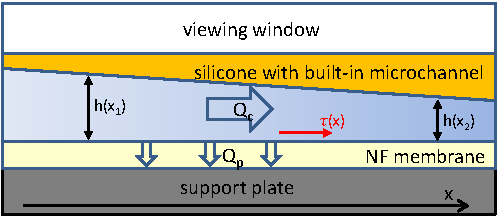
\includegraphics[width=0.6\textwidth]{figures/introduction/figure1_3}%
\caption{Concept schematic design of the microfluidic platform.}%
\label{figure1_3}%
\end{figure}

\begin{enumerate}
	\item Novel processing techniques development for silicone microchannel design and fabrication.
	\item Present a design of a novel modular reusable and resealable microfluidic platform which fulfills the following requirements:
	\begin{enumerate}
	\item Housing design which contains connection interfaces for injecting and discharging fluids;
	\item Flexible designed microchannels integrated in the platform;
	\item Optical transparent viewing window which allows direct investigation of the flow in the microchannel.
    \end{enumerate}
	\item Operative at high pressure (up to 10bar).
	\item Design and fabrication of the pressure and leakage test setup, pressure and leakage test of the setup.
\end{enumerate}

In the first aim we decided to develop a novel processing technique for fabricating microchannels in silicone membranes. This new rapid prototyping process should be flexible and avoid any cleanroom processes in order to save the lead times and cost. This new process should also provide proper processing precision.\\

In the second aim the preliminary microfluidic platform is designed to integrate the microchannel and the nanofiltration membranes. This part is critical because the design needs to be mechanically stable to meet the high pressure testing environment and no leakage is allowed to present at the macro-to-micro connection interfaces.\\

Then the housing of the microfluidic platform and all part which will be integrated into it are fabricated. A test setup is also designed and fabricated to pump test fluid into the platform. Pressure and leakage tests are conducted and must provide experimental results which indicate that the designed microfluidic platform is able to operate under high pressures and new improvements of the design are made according to the test results.

\subsection{Structure of This Work}
\label{1_2_2}
This master thesis is presented in five chapters. In \autoref{2} a short review on the microfluidic platforms for lab-on-a-chip applications is illustrated. Since the design in this master thesis is for high pressure applications, some state-of-the-art technologies about sealing and packaging for such applications are also explained.\\

In \autoref{3} the design and fabrication steps for every part in the preliminary design are introduced. Some details about nanofiltration membranes are presented at first. Then, the reasons for the choosing of silicone as the microchannel layer are explained by presenting two main advantages regarding the material properties and the corresponding processing technology. The fabrication of the silicone membrane and the microchannel processing technique are presented in details since this processing technique in not standard process. Finally, the housing design of the microfluidic platform is shown and the design of the pressure and leakage test setup is explained.

\begin{figure}[h]%
\centering
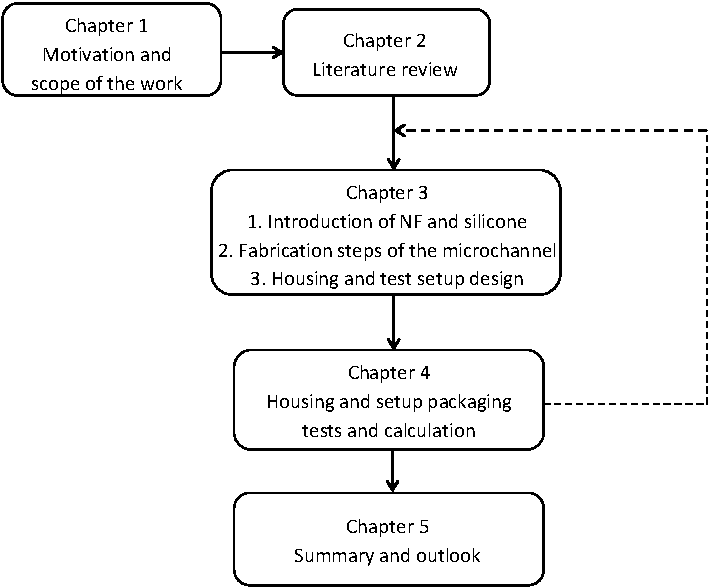
\includegraphics[width=0.8\textwidth]{figures/introduction/figure1_4}%
\caption{Work flow for reaching goals of the master thesis. The dash line shows the iterative steps to improve the performance of the design depending on the former test results.}%
\label{figure1_4}%
\end{figure}

\autoref{4} provides the packaging of both the chip housing and the test setup. In this chapter, the results of the pressure and leakage test with different housing design are presented and compared. The throughput of the flow and the filtration efficiency based on the last housing design is also calculated. In the last chapter the test results are discussed and the achievements in this thesis work are summarized. Finally, a brief overview over the further possibilities to improve the microfluidic platform design and the test setup is presented.